\section{Assignment 6}

\subsection{Design the joint space PD control law with gravity compensation}

The goal is to implement the following architecture:

\begin{figure}[h]
\centering
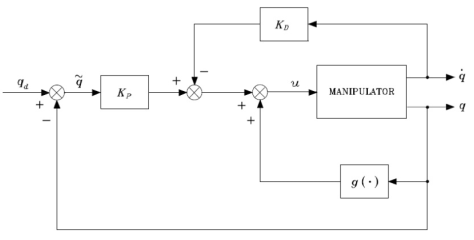
\includegraphics[keepaspectratio,width=0.4\textwidth]{joint_PD_arch}
\caption{Joint space PD control law with gravity compensation architecture}
\end{figure}

The architecture follows the control law:

\begin{equation*}
\tau = g(q) + K_P(q_d-q) + K_D(\dot q_d -q_d)\;\;\;\;\;\text{with }K_P = 50,K_D =  10
\end{equation*}

The architecture was implemented in SIMULINK as follows:

\begin{figure}[h]
\centering
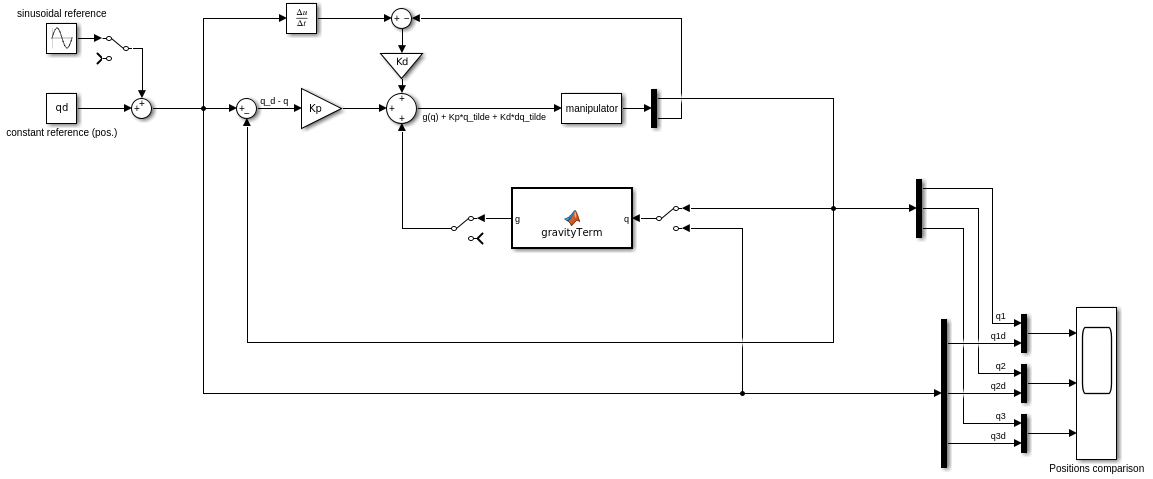
\includegraphics[keepaspectratio,width=0.6\textwidth]{joint_PD}
\caption{Joint space PD control law with gravity compensation SIMULINK model}
\end{figure}

\begin{figure}[H]
\centering
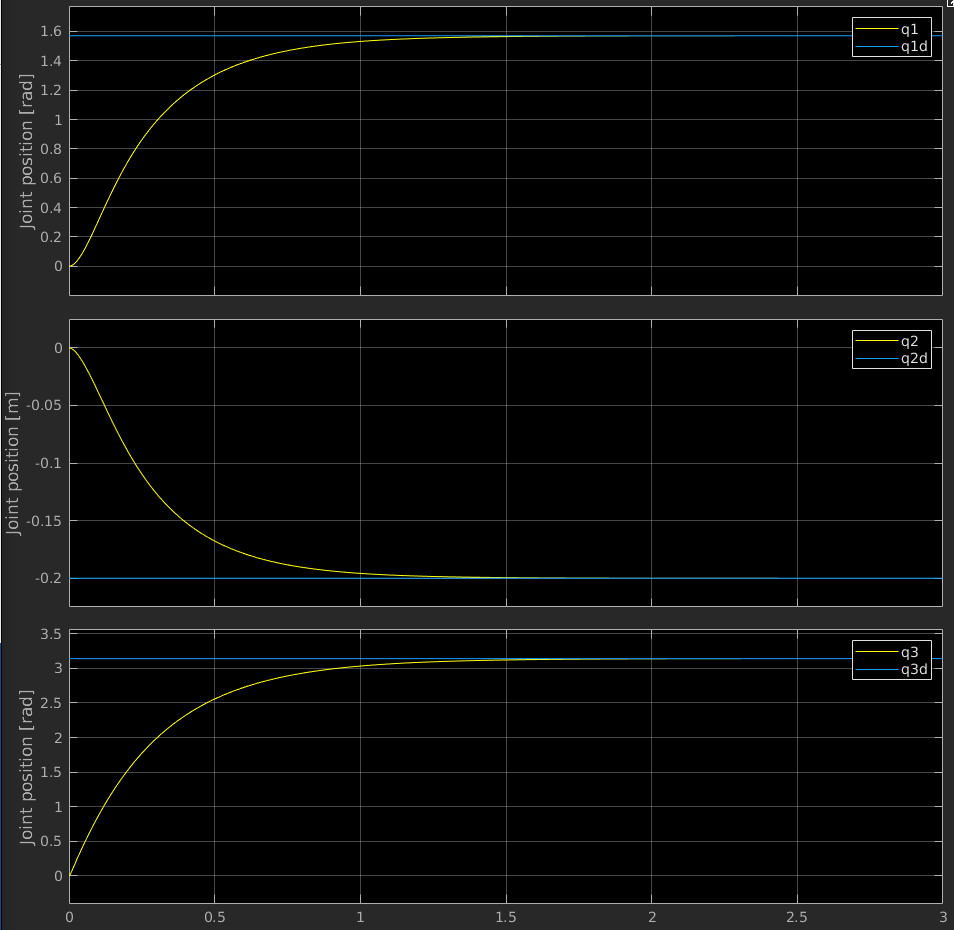
\includegraphics[keepaspectratio,width=0.5\textwidth]{joint_PD_correct}
\caption{Joint positions - constant reference $q_d=\begin{bmatrix}
\pi/2& -0.2& \pi\end{bmatrix}^T$}
\end{figure}

\subsection{What happens if g(q) is not taken into account?}

\begin{figure}[H]
\centering
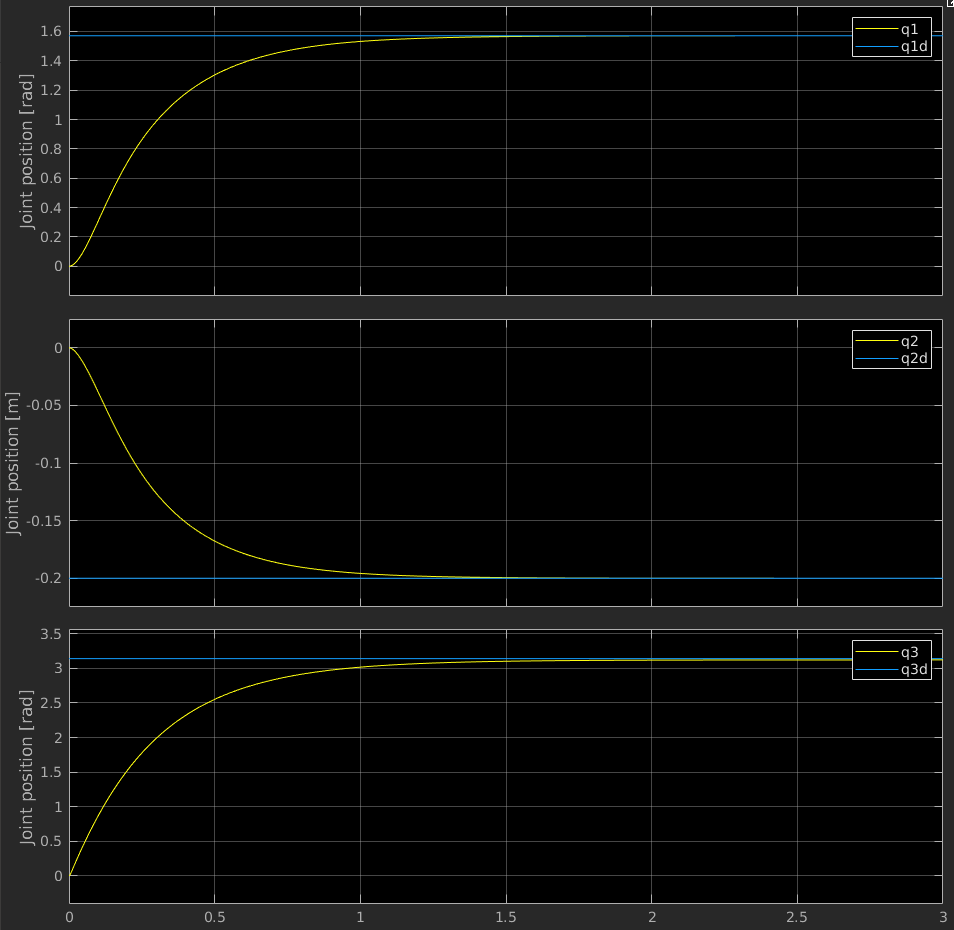
\includegraphics[keepaspectratio,width=0.6\textwidth]{joint_PD_nog}
\caption{Joint positions - $g(q)=0$}
\end{figure}

\subsection{What happens if the gravity term is equal to g($q_d$)?}


\begin{figure}[H]
\centering
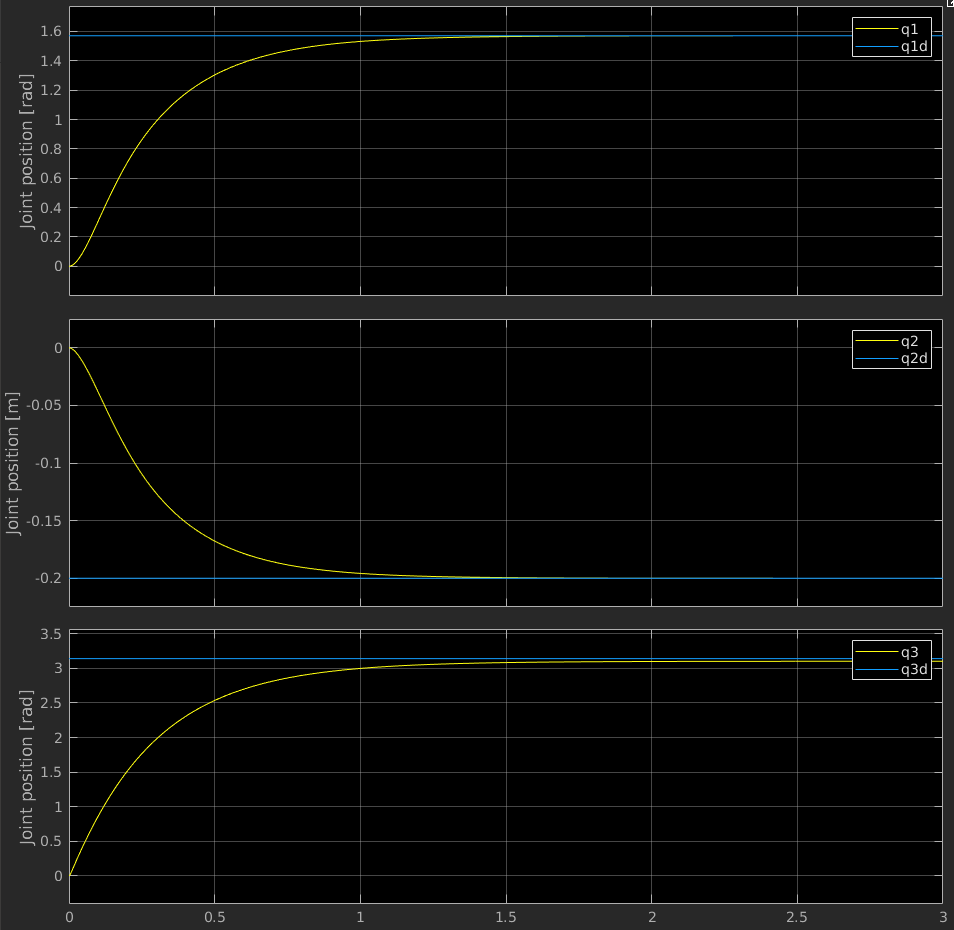
\includegraphics[keepaspectratio,width=0.6\textwidth]{joint_PD_wrongg}
\caption{Joint positions - $g(q)=g(q_d)$}
\end{figure}

\subsection{What happens if $q_d$ is not constant?}


\begin{figure}[H]
\centering
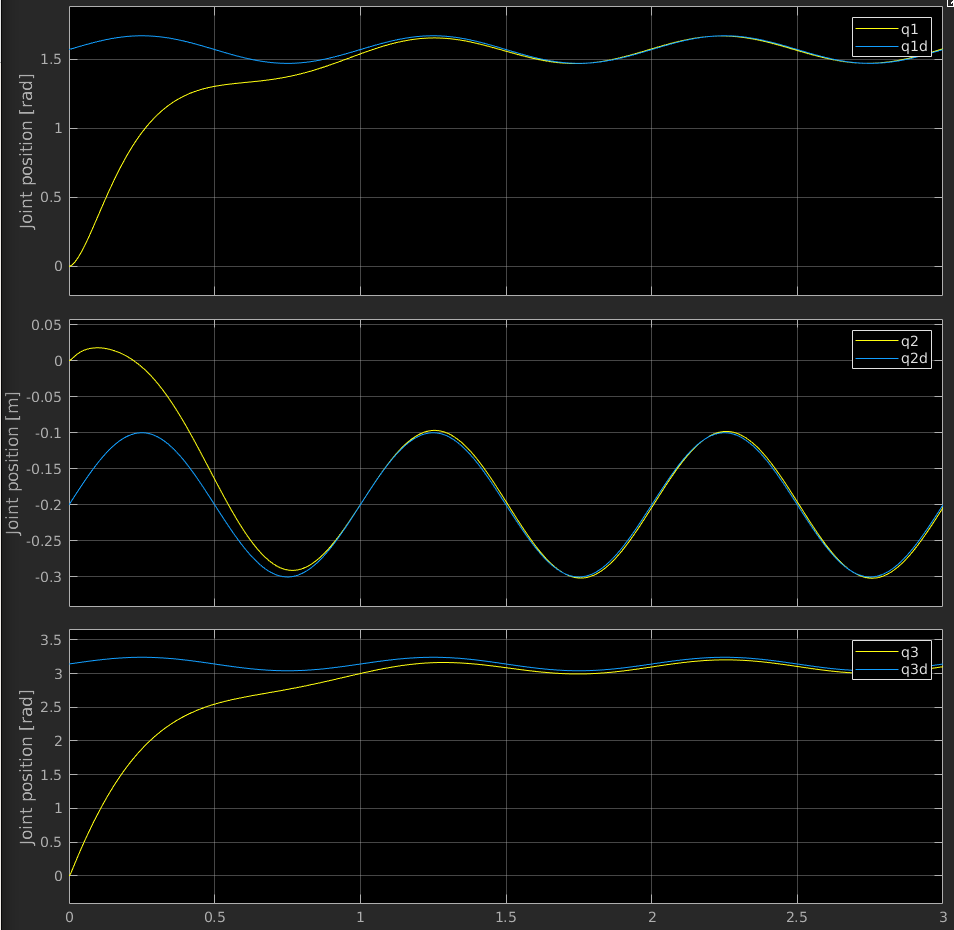
\includegraphics[keepaspectratio,width=0.6\textwidth]{joint_PD_sin}
\caption{Joint positions - sinusoidal reference $q_d = \begin{bmatrix}
\pi/2& -0.2& \pi
\end{bmatrix}^T + 0.1sin(2\pi)$}
\end{figure}
